The {\it Regularization Loss} $\cL_{\rm {reg}}$ is inspired by the Hessian-based Locally Linear Embedding (HLLE) model~\cite{ai.Donoho2003} and minimizes the Frobenius norm of the Hessian of deformation over a specified input volumetric space. This approach is based on the property that a vanishing Hessian guarantees locally isometric deformations, preserving the local geometric structure and effectively implementing the deformation as a rigid transformation, thus maintaining mesh quality.
In practice, we treat the input template CFD mesh a discretization of an isotropic Euclidean coordinate space, where its tangent space is identical to the input coordinate space itself. DeepGeo's Hessian at an arbitrary position $\bv$ can be calculated with the Cartesian coordinate system as:
%
\begin{small}
\begin{align}
       \bH \left( \bv \right) 
      = \begin{bmatrix}
            \frac{\partial^2 \bv}{\partial x^2} & \frac{\partial^2 \bv}{\partial xy} &  \frac{\partial^2 \bv}{\partial xz} \\
            \frac{\partial^2 \bv}{\partial xy} & \frac{\partial^2 \bv}{\partial y^2} &  \frac{\partial^2 \bv}{\partial yz} \\
            \frac{\partial^2 \bv}{\partial xz} & \frac{\partial^2 \bv}{\partial yz} &  \frac{\partial^2 \bv}{\partial z^2} \\
        \end{bmatrix} \; .
\end{align}
\label{ch5:eq:L_reg} 
\end{small}
%
DeepGeo relies on a loss term that minimizes the quadratic form of Hessian as $\int_{\mathfrak{C}} \left\| \bH(\mathit{c})) \right\|^2_F d\mathit{c}$, where $\mathfrak{C}$ is the subset of input coordinate space bounded by $\hat{V}^V$ that defines the CFD computational domain.
This quadratic term measures DeepGeo's average ‘curviness’ over $\mathfrak{C}$.
To further speed up the computation and due to the inherent generalization ability of neural networks, $\cL_{\rm reg}$ can estimated by evaluating the Hessian only on a finite and small number of vertices sampled from $\hat{V}^V$, enabling efficient computation via auto-differentiation.
Minimizing $\cL_{\rm reg}$ directly provides an adjoint approach for optimization, and is considerably simpler than finding the Hessian’s null space and corresponding basis vectors as required in the original HLLE.

Fig.~\ref{ch5:fig:w_loss_reg_ablation} illustrates the effectiveness of the $\cL_{\rm reg}$ regularization. In this example, the template mesh $\hat{M}$ is a RAE-2822 airfoil while the target shape $S$ is the same airfoil rotated by 45 degrees, imitating a large spanwise twist for 3D wing design. Without regularization, the deformed CFD mesh $M$ exhibits severe defects, such as overlapping cells and high non-orthogonality, as shown in Figure~\ref{ch5:fig:w_loss_reg_ablation}(b). As the regularization weight $\lambda_{\text{reg}}$ is progressively increased, these issues are resolved and the quality of $M$ closely eventually matches that of $\hat{M}$, as shown in Figure~\ref{ch5:fig:w_loss_reg_ablation}(c-d).

\begin{figure}[ht]
    \begin{center}
        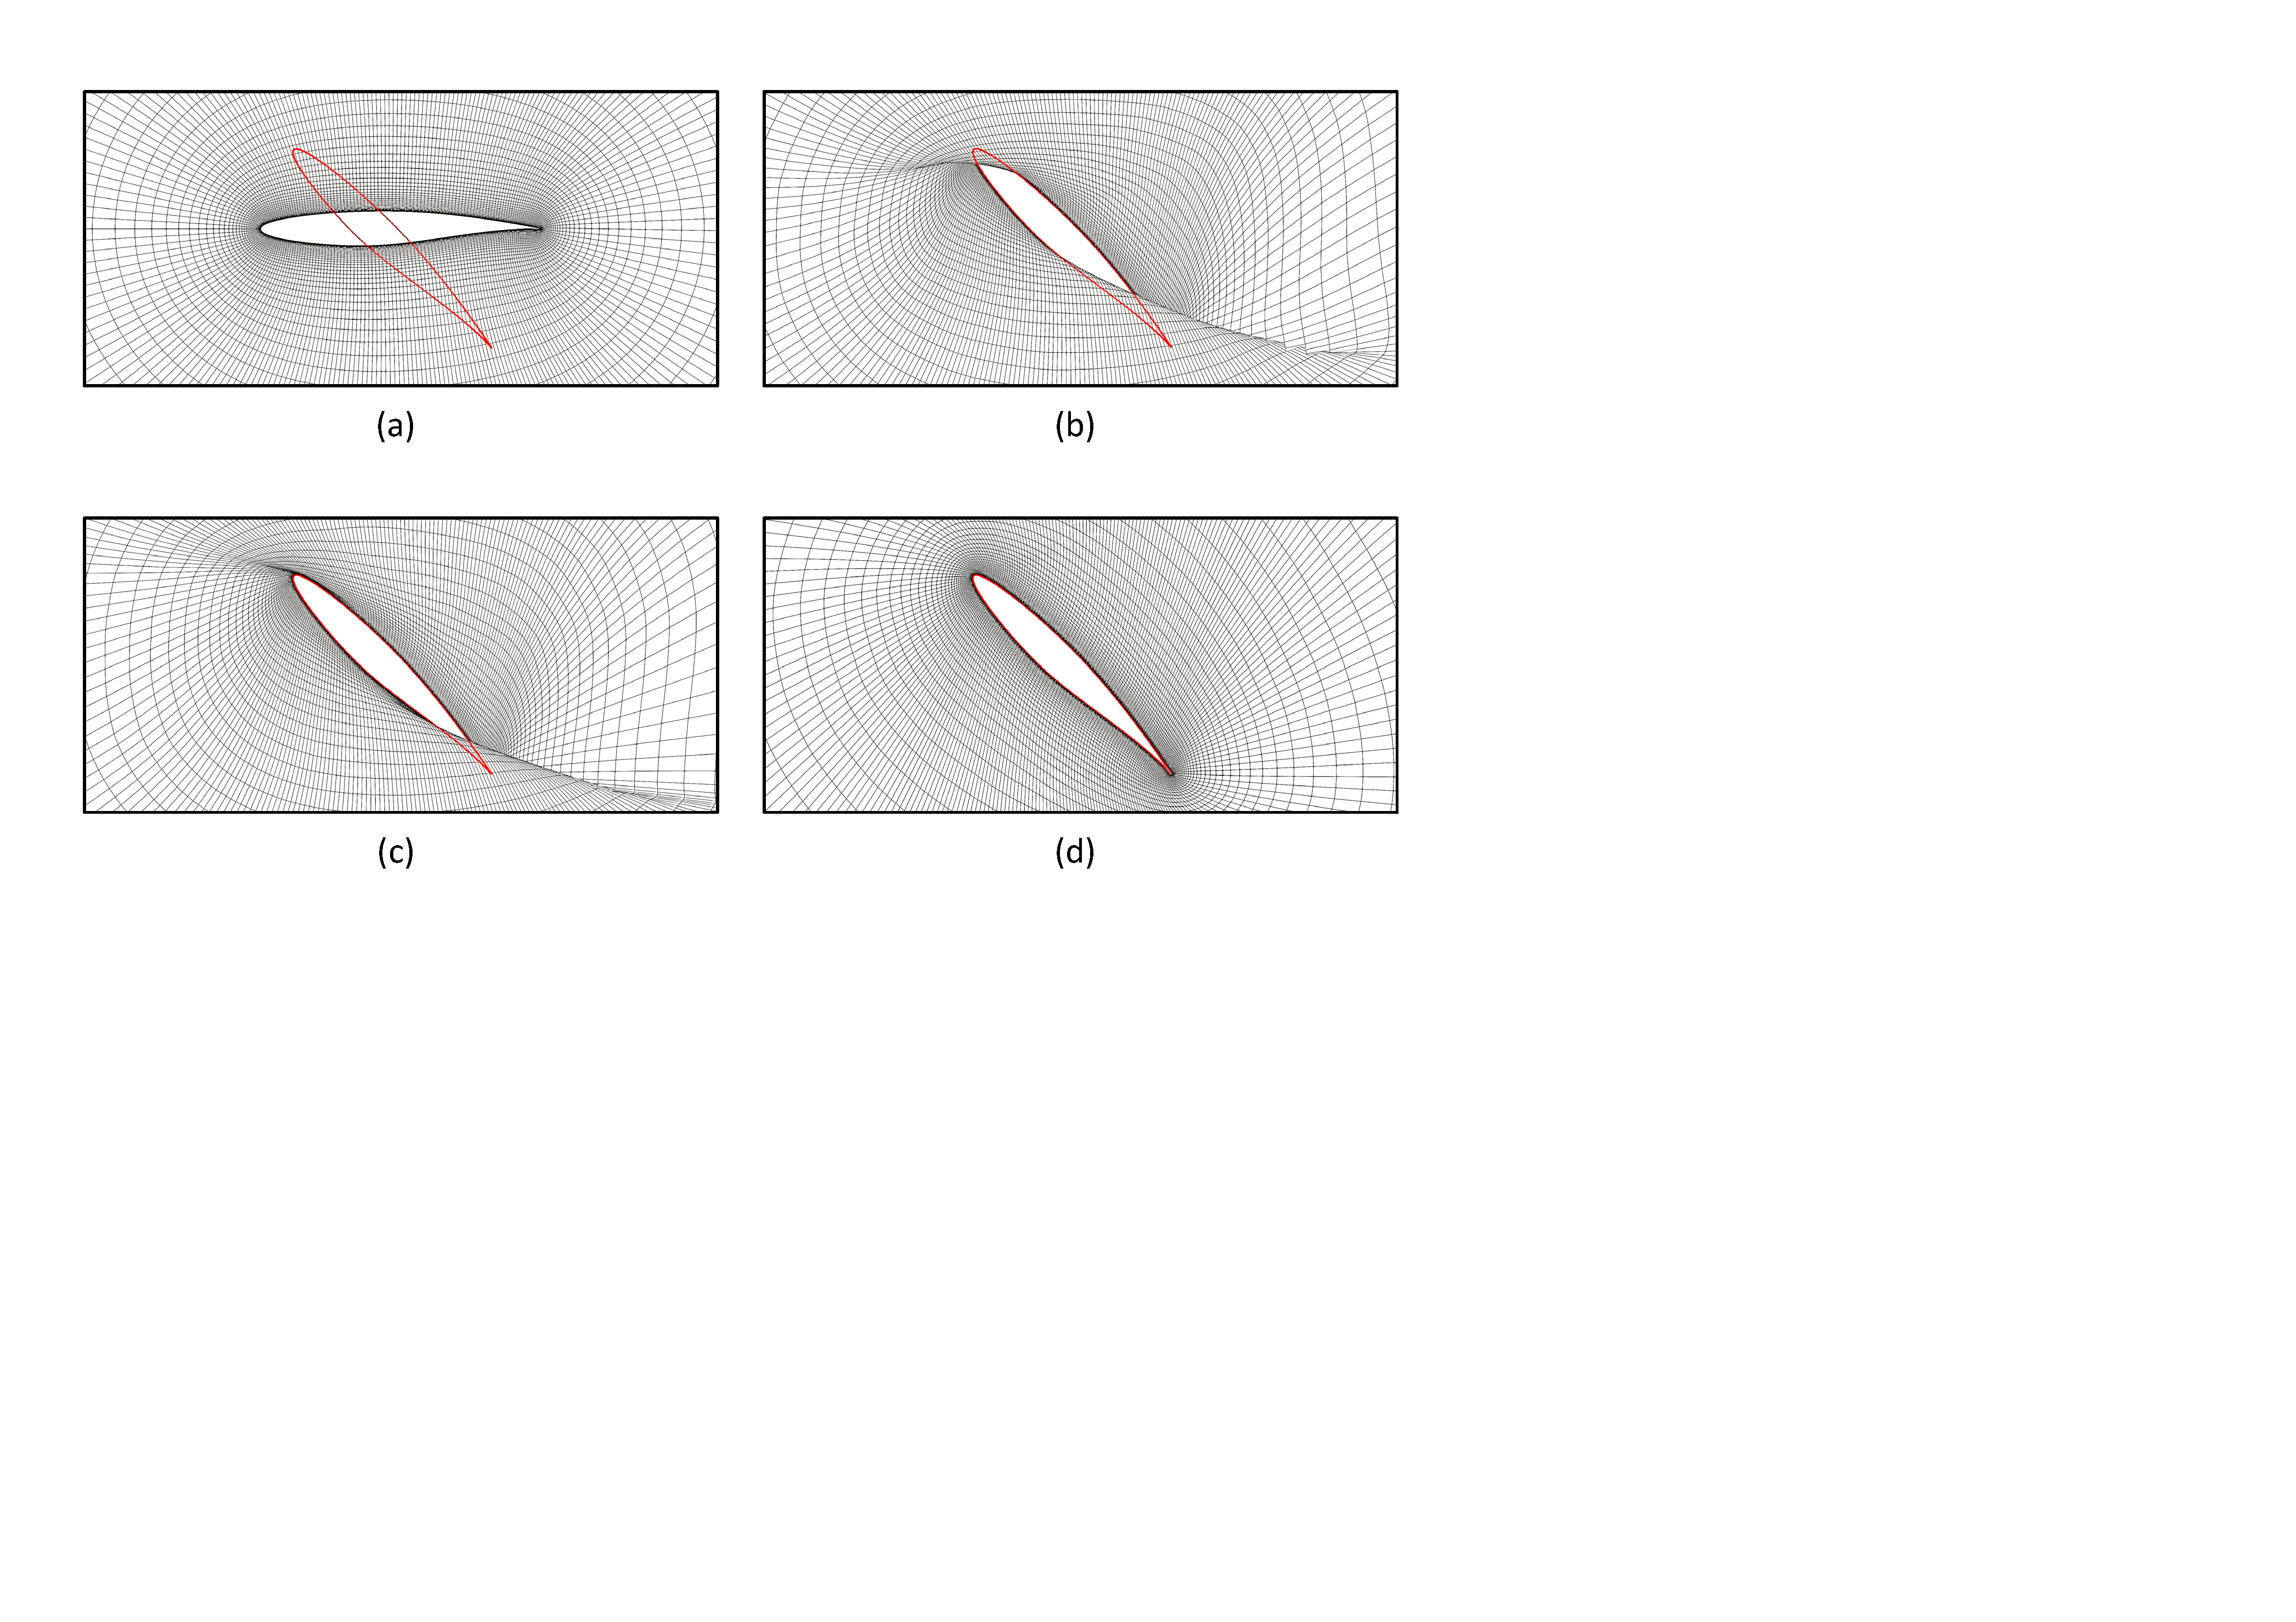
\includegraphics[width=1\linewidth]{chapter5/fig/journal_ablation_studies_w_loss_reg.pdf} 
    \end{center}
    \caption{
        \small \textbf{ Investigation of $\cL_{\rm reg}$ by deforming the mesh in black to fit the shape in red, as shown in (a), with (b) $\lambda_{reg}$=0, (c) $\lambda_{reg}$=10 and (d) $\lambda_{reg}$=100.}
        %Effectiveness of the regularization}  $\cL_{\rm reg}$. 
        %(a) The investigation starts with the template mesh $\hat{M}$ in black and the target shape $S$ in red. 
        %(b) It shows deformation without regularization ($\lambda_{reg}$=0). Severe mesh issues such as overlapped cells and high nonorthognality appear.
        %(c) With $\lambda_{reg}=10$, the mesh quality improves.
        %(d) With $\lambda_{reg}=100$, the mesh issues are removed and the deformed mesh has comparable quality for simulation as that of the original template mesh.
    }
    \label{ch5:fig:w_loss_reg_ablation}
\end{figure}

%-------
% OLD
%--------

\iffalse

The $\cL_{\rm reg}$ implements an isometric mapping of $\mathbb{R}^3 \rightarrow \mathbb{R}^3$ by developing from the 
The goal of HLLE model is to reconstruct a mapping such that the Hessian vanishes at the input coordinates. 
This vanishing Hessian guarantees the mapping outputs the isometric coordinates in the deformed space, preserving the local geometric structure of the manifold.
To this end, we regard the input template CFD mesh as a discretization of an isotropic Euclidean coordinate space.
The tangent space is identical to the input coordinate space itself.
DeepGeo's Hessian at an arbitrery position $\bv$ can be efficiently calculated with the Cartesian coordinate system, defined as
\begin{small}
\begin{align}
       \bH \left( \bv \right) 
      = \begin{bmatrix}
            \frac{\partial^2 \bv}{\partial x^2} & \frac{\partial^2 \bv}{\partial xy} &  \frac{\partial^2 \bv}{\partial xz} \\
            \frac{\partial^2 \bv}{\partial xy} & \frac{\partial^2 \bv}{\partial y^2} &  \frac{\partial^2 \bv}{\partial yz} \\
            \frac{\partial^2 \bv}{\partial xz} & \frac{\partial^2 \bv}{\partial yz} &  \frac{\partial^2 \bv}{\partial y^2} \\
        \end{bmatrix}
\label{ch5:eq:L_reg} 
\end{align}
\end{small}
, DeepGeo relies on a loss term that minimizes the quadratic form of Hessian as $\int_{\mathfrak{C}} \left\| \bH(\mathit{c})) \right\|^2_F d\mathit{c}$, where $\mathfrak{C}$ is the subset of input coordinate space bounded by $\hat{V}^V$ that defines the CFD computational domain.
This quadratic term measures DeepGeo's average ‘curviness’ over $\mathfrak{C}$.
Thanks to neural network's generalization ability, $\cL_{\rm reg}$ can effectively implement the quadratic form of Hessian by only sampling a finite and small number of vertices from $\hat{V}^V$, resulting in the form as in Eq.\ref{ch5:eq:losses}.
\WZ{Let me know if a small ablation study is still needed.}

\fi